% !TEX root = ../main.tex

\section{Introduction}
    \vspace{-0.5ex}

    %* show the problem
    %* introduce the idea
    %* contributions?

%% motivation
Extending the capabilities of robots for providing services in complex human environments has become a popular field of research.
In this domain, perception capabilities such as recognizing objects in a scene are crucial to reliably perform service tasks in various conditions.
%% challenges
Current state-of-the-art object recognition systems recognize objects based on static images~\cite{tang2012textured,van2013fusing}.
However, these systems prove limited in cases when objects are in ambiguous orientations or distinctive features are hidden due to the pose of the object.

%% related work
%% active perception    
A popular approach to tackle this problem is active perception~\cite{atanasov2013hypothesis}, where the robot is intelligently moving its camera to reveal more information about the scene.
However, there are many cases where this approach will fail, since distinctive features may be hidden, for example, on the bottom side of the object (see \figref{fig:pr2}).
%% interactive perception: segmentation
The complementary idea of a robot interacting with the scene to improve its perceptual capabilities by revealing informative surfaces has been particularly explored in the area of segmentation.
Examples are the interactive segmentation of rigid objects being moved by a robot~\cite{KenneyInteractive}, the segmentation of articulated objects~\cite{Katz-WS-MM-ICRA2011}, and the disambiguation of segmentation hypothesis~\cite{bergstrom11icvs}.
All these approaches, however, do not reason about what actions to take in order to achieve the goal.

%% approach
In this work we introduce a probabilistic method for choosing object manipulation actions to optimally reveal information about objects in a scene based on the robot's observations.
To the best of our knowledge, the problem of interactive object recognition has not been addressed before. 
Our novel approach enables a robot to interact with objects and adjust their pose to reveal discriminative features for determining their identity.
In the ambiguous book example (see~\figref{fig:pr2}), this means flipping the book over and observing the cover, which results in more confident recognition.
Our method is based on a probabilistic graphical model for feature-based object and pose recognition.
By inferring posterior distributions of object probabilities conditioned on all previous actions and observations, our approach enables a robot to select the optimal action to reduce the uncertainty of object recognition.

%% contributions
The key contributions of this approach are that (a) it presents a probabilistic action selection model that reasons about the most informative action, which leads to optimality in the number of actions to recognize the object and (b) it takes into account a probabilistic object recognition model that is independent of the feature type.



    \setlength{\tabcolsep}{0.1em}
    \begin{figure}[ht]
    \begin{tabular}{cccc}
    \multicolumn{2}{c}{\multirow{-5}{*}{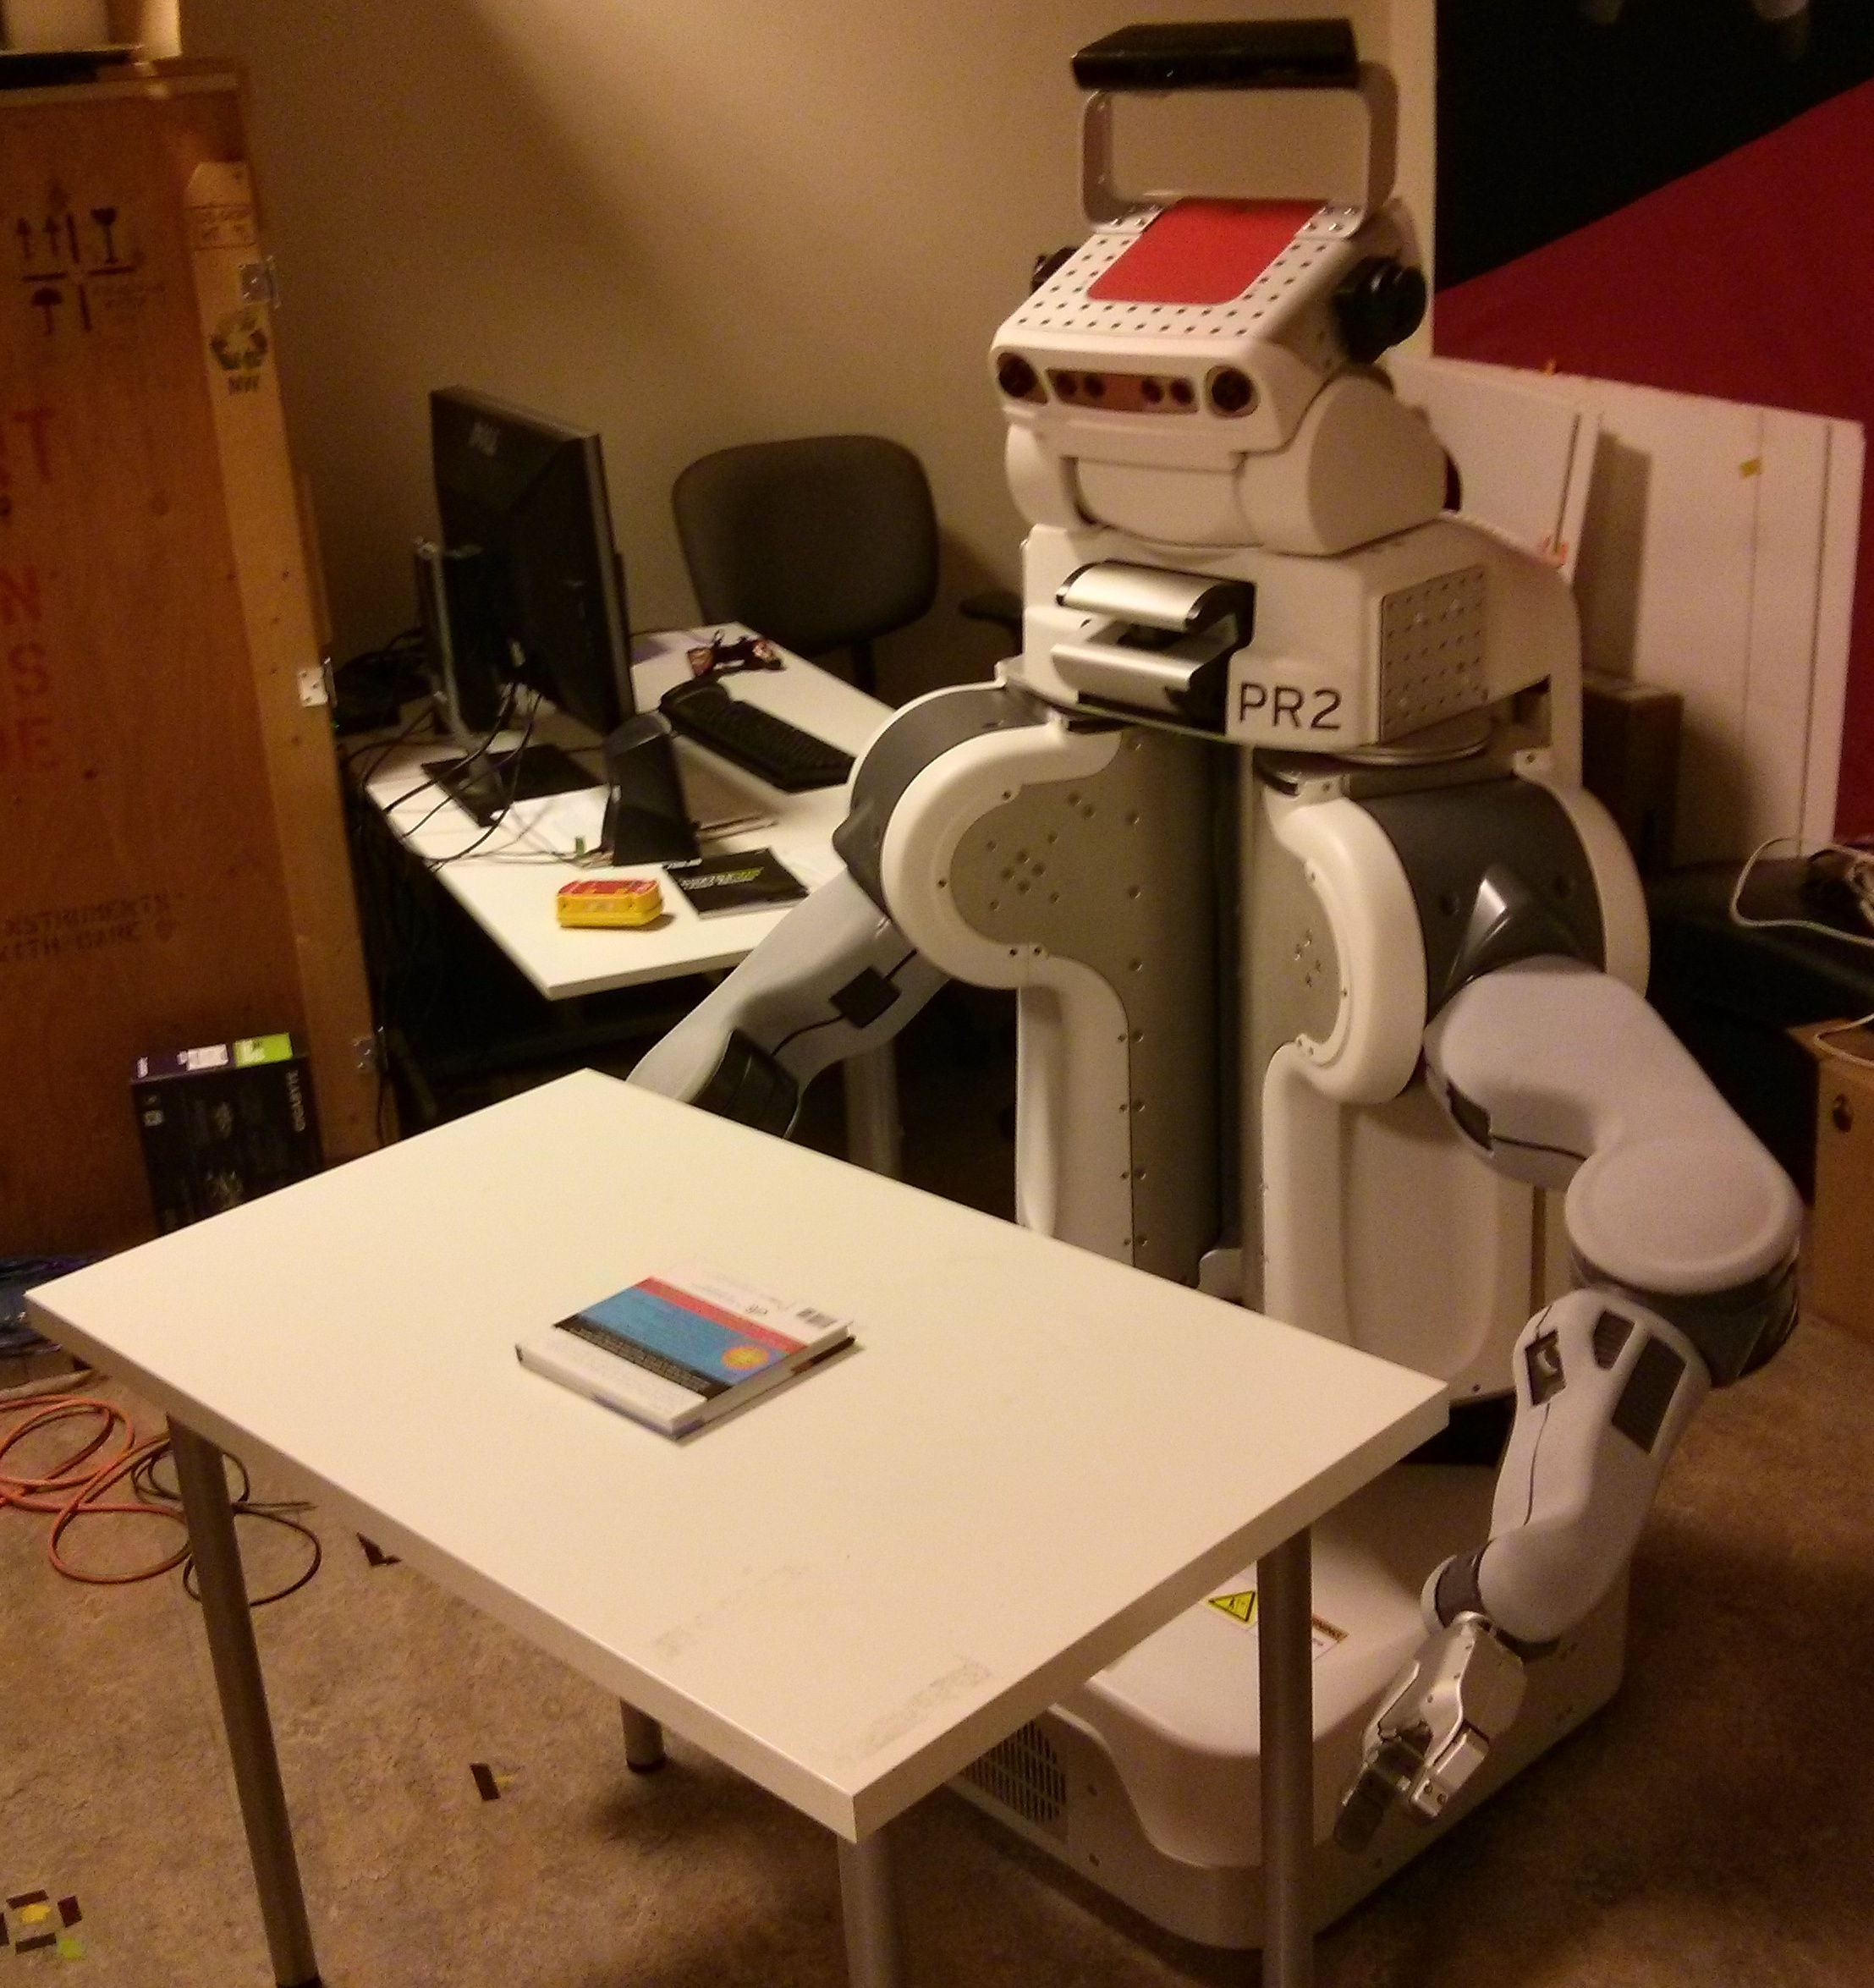
\includegraphics[width=0.46\columnwidth]{pics/pr2_init.jpg}}} & \multicolumn{2}{c} {\begin{overpic}[width=0.46\columnwidth]{pics/first1.jpg} 
    \put(40,46){Book 1}
    \end{overpic}}\\
    %&
\includegraphics[width=0.23\columnwidth]{pics/first_cover1.jpg} \\
    \multicolumn{2}{c}{} &  \multicolumn{2}{c} {\begin{overpic}[width=0.46\columnwidth]{pics/first2.jpg} 
    \put(40,46){Book 2}
    \end{overpic}} \\
    \multicolumn{2}{c}{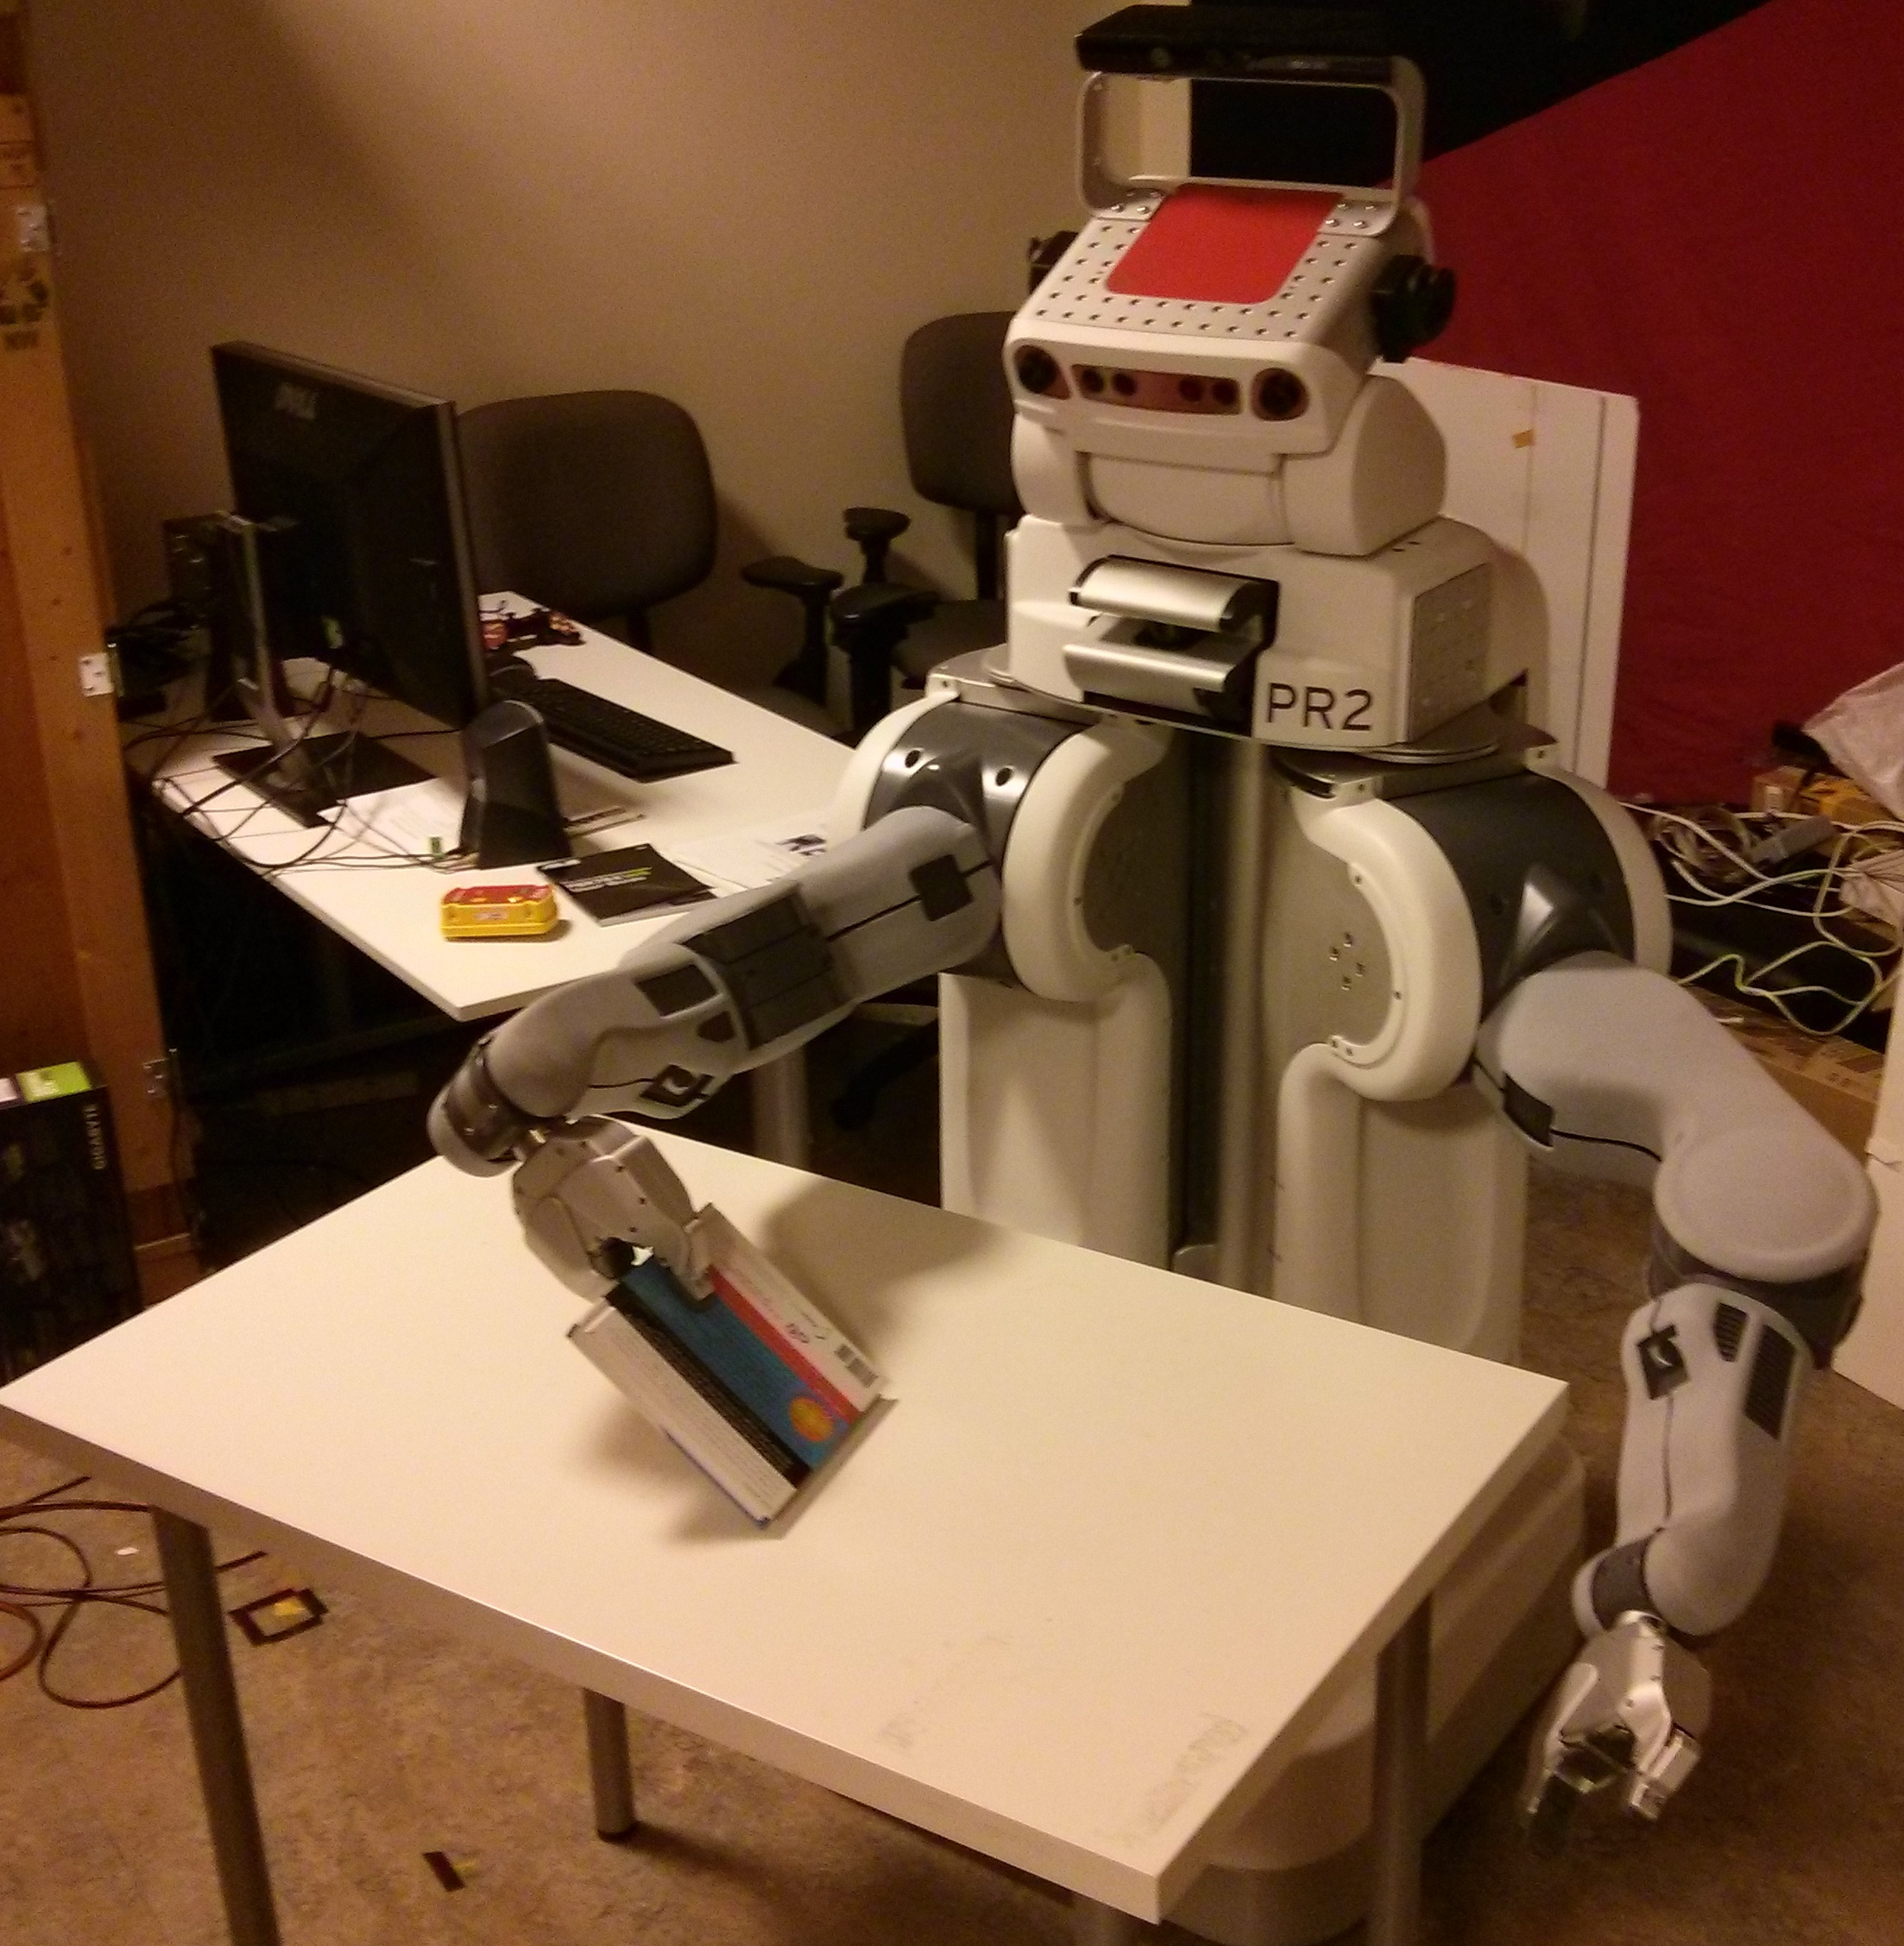
\includegraphics[width=0.45\columnwidth]{pics/pr2_grasp.jpg}}
    & \multicolumn{2}{c}{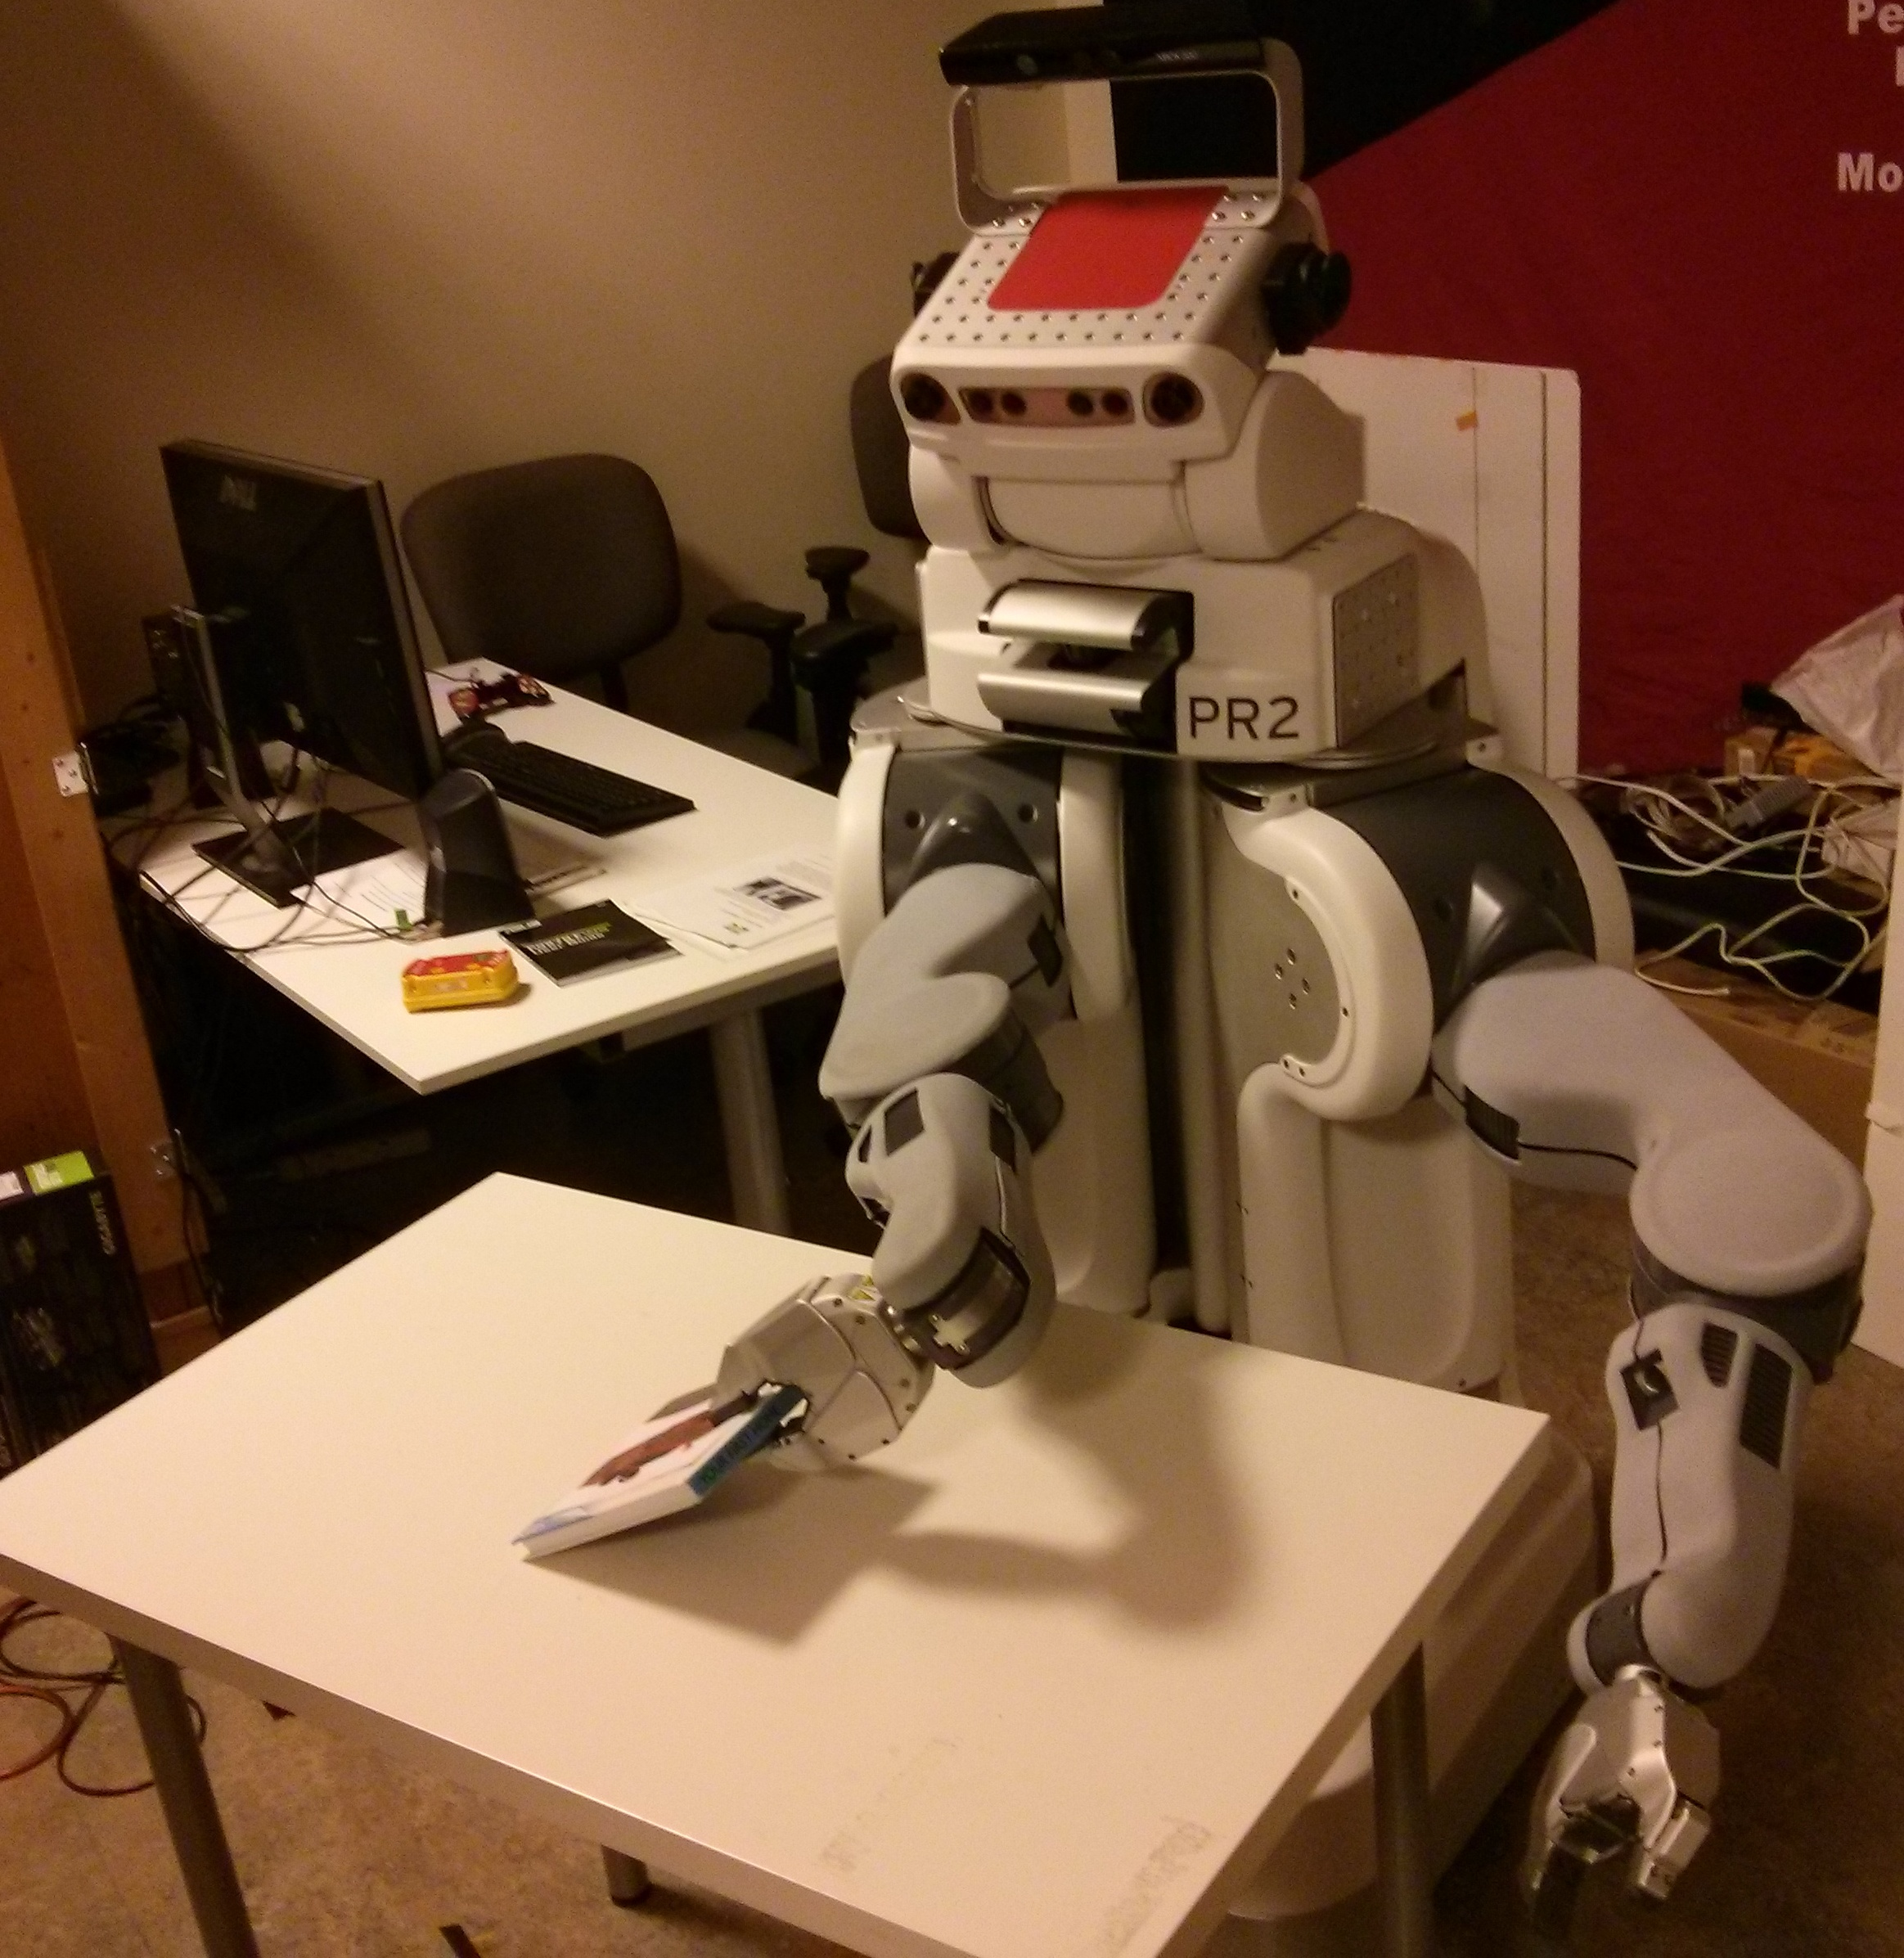
\includegraphics[width=0.45\columnwidth]{pics/pr2_rotate.jpg}}
    \end{tabular}
    \caption{Top-left: The service robot PR2 trying to recognize a book based on its back. The database of objects consists of book 1 (top-right, NE and NW) and book 2, (top-right, SE and SW) that look the same from the back. PR2 takes the optimal action in order to recognize which book it is. In this case it means it flips it over (bottom-left, bottom-right).}
    \vspace{-4ex}

    \label{fig:pr2}
    \end{figure}

    %contributions
    %* novel probabilistic model for object recognition
    %* action selection probabilistic algorithm to pick the optimal action in order to recognize the object
